\section{Introduction}
Electricity usage permeates all aspects of modern society.
Its most conspicuous
uses include urban contexts such as
lighting, air conditioning, refrigeration, heating, and, powering
appliances and gadgets but its penetration is pervasive across rural
and industrial sectors.
In 2013, the residential and commercial sector
comprised nearly 40\% of all the electricity generated in the U.S.~\cite{energydatabook2011}.
Furthermore, our dependence on electricity will continue to grow
as emphasis shifts away from fossil fuel based vehicles to electric
vehicles.

While people generally agree on the importance of conservation and
usage curtailment, they are often at difficulties to quantify 
{\em where, when} and {\em how much} electricity is consumed.
Typically, residences and businesses receive
monthly electricity bills indicating aggregate usage, with no information on
the breakdown of consumption by appliances/devices, time of day, or day of
week (this is an area in great flux, however). Research has 
shown that simply making such feedback available to users
can reduce consumption by up to 50\%, although typical savings
are in the 9\% to 20\% range~\cite{energydatabook2011}.


%In modern society, people prefer a comfortable life at home,
%at work and  during leisure time outside.
%Energy, such as electricity, gas, bring us convenience in our daily lives.
%However, the use of energy causes environment pollution as well.
%Energy consumption increases continuously even faster than the population.
%One challenge we are facing is how to effectively
%save and easily manage energy usage at home \cite{cook2012smart},
%in office and in plants.

One obvious approach to determining the breakdown of consumption is to install
power meters in every circuit (and subcircuit)
to capture consumption of individual devices in homes and
offices. Such installation is costly and intrusive, making 
this option unviable in practice. 
An alternate
solution, called energy disaggregation or non-intrusive load monitoring
(NILM),
first proposed by Hart~\cite{hart1992}, is to use analytics to 
{\em infer} the breakdown of consumption from an aggregate 
power measurement of a
site. This drastically reduces the number of meters required per 
home/installation, typically to just one. Furthermore, depending on the analytics desired, it is possible to
use the measurements already being recorded by a utility meter for
disaggregation, especially in cases where utility companies have deployed
smart meters.

Energy disaggregation is hence today a booming area offering both
challenging problems for data analytics and having practical relevance in a
number of areas including sensor networks and building analytics.
Our goal in this paper is to provide a comprehensive survey of recent
advances in the area of energy disaggregation with a focus on the data mining
and machine learning algorithms used. 

%% The approaches applied to NILM not only discover the usage pattern of electricity, but also the techniques it uses can be applied to
%% water disaggregation  and
%% gas disaggregation \cite{froehlich2011disaggregated}.
%% Since this research helps conserve various resources from all perspectives,
%% it becomes more and more significant and popular in recent years.

\subsection {Background}

Hart~\cite{hart1992} first proposed the idea that power measurements at the
main electric meter in a home can be used to deduce what appliances are
turned on and how much electricity they are consuming.
Figure~\ref{fig_energyDisaggDefinition} (a) shows aggregate power measurement,
such as that at a main electric meter, from 10 am to 12 noon on a particular
day. The goal of energy disaggregation is to decompose this consumption into
its constituents as shown in Figure~\ref{fig_energyDisaggDefinition} (b),
which shows fourteen disaggregated devices. It shows that, for example, the
refrigerator turns on twice -- from 10:15 am to 10:40 am, and then from 11:50
am to 12:00 noon. At other times, the refrigerator stays off.

%shows an example of energy
%disaggregation by only recording the power usage of two main entry lines which
%are connected to a residential building \cite{kolter2010redd}. 
%\manishc{in fig 1 show two figures, the first with only the aggregate
%  consumption, the second with the disggregated components as you already
%  have. To make it fit, you can make the current figure shorter, perhaps
%  starting it around 10am (also put 'am' in the x-axis labels)}
%% Through disaggregation, we can find from Figure\ref{fig_energyDisaggDefinition} (b) that 
%% there are fourteen aggregated devices in total from 8:00am to 12:00am on a given day.
%% We aim to find out the status of these fourteen devices.
%% For example, the refrigerator is on during three periods: 8:50am to 9:05am,
%% 10:15am to 10:40am, and 11:50am to 12:05pm.
%% During other times, the refrigerator is off.


\begin{figure*}[ht]
	\centering{
    \begin{tabular}{cc}	
    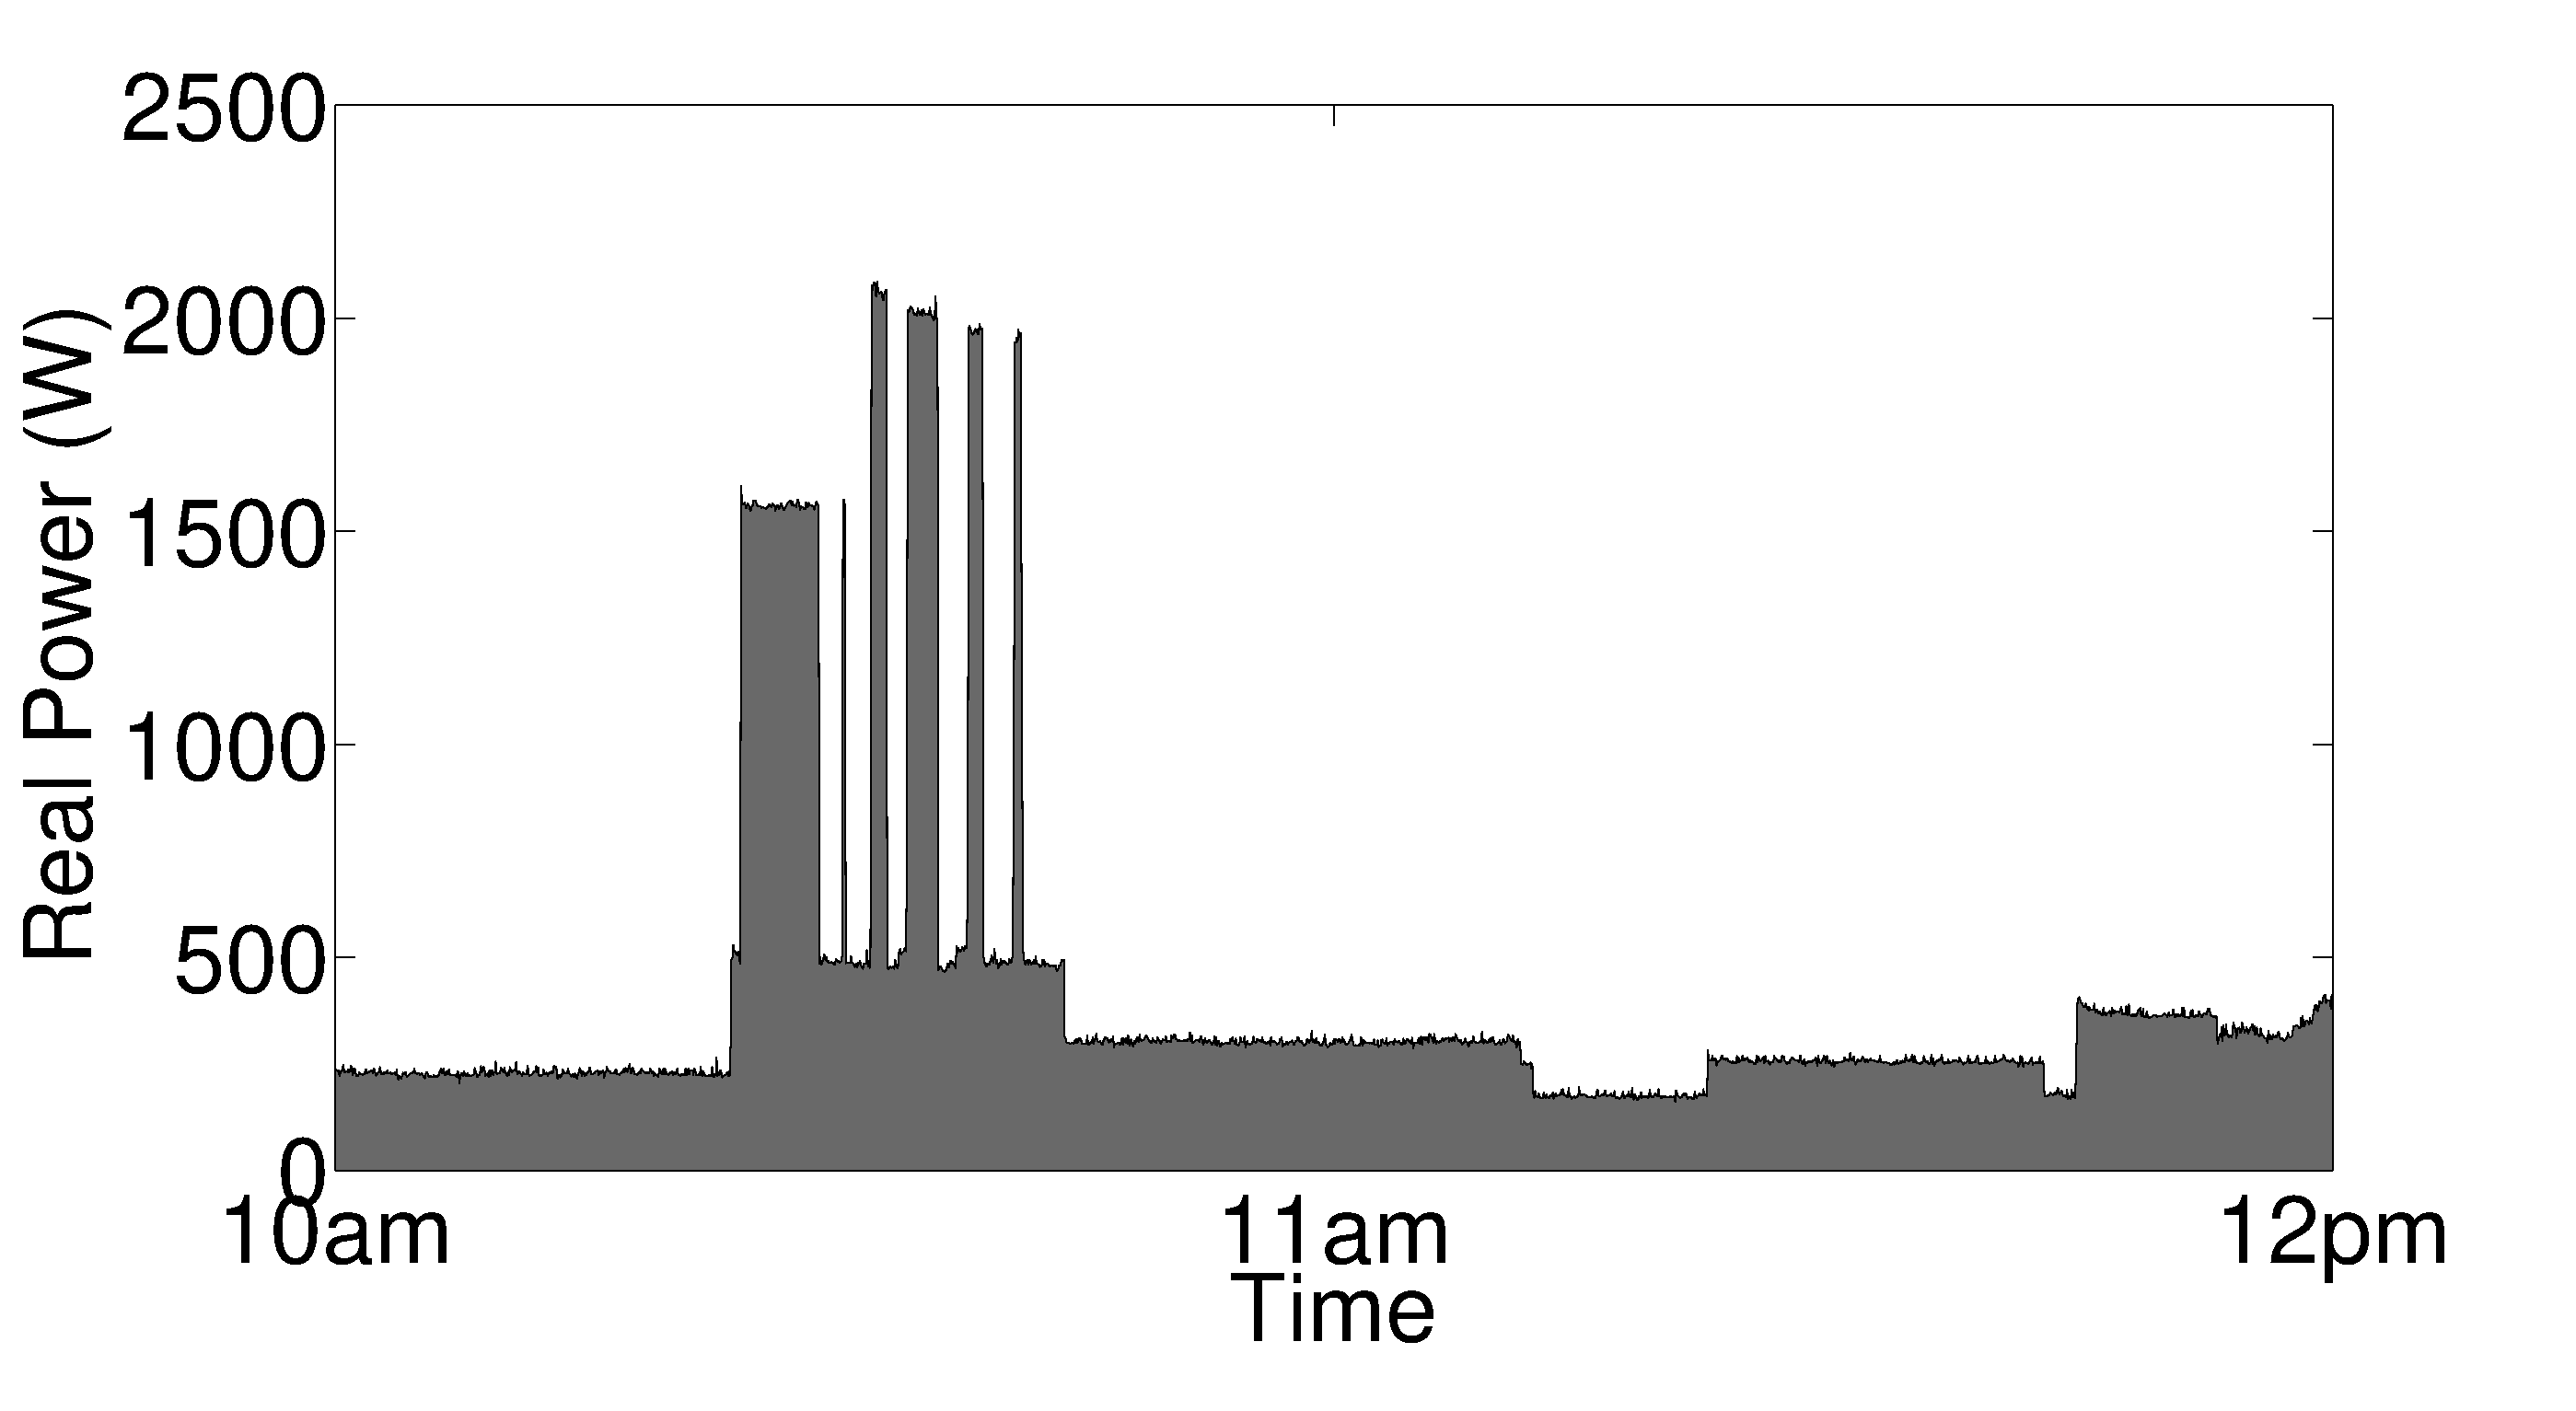
\includegraphics[width=0.5\textwidth]{figs/truth_agg.pdf}\hspace{1em}&
	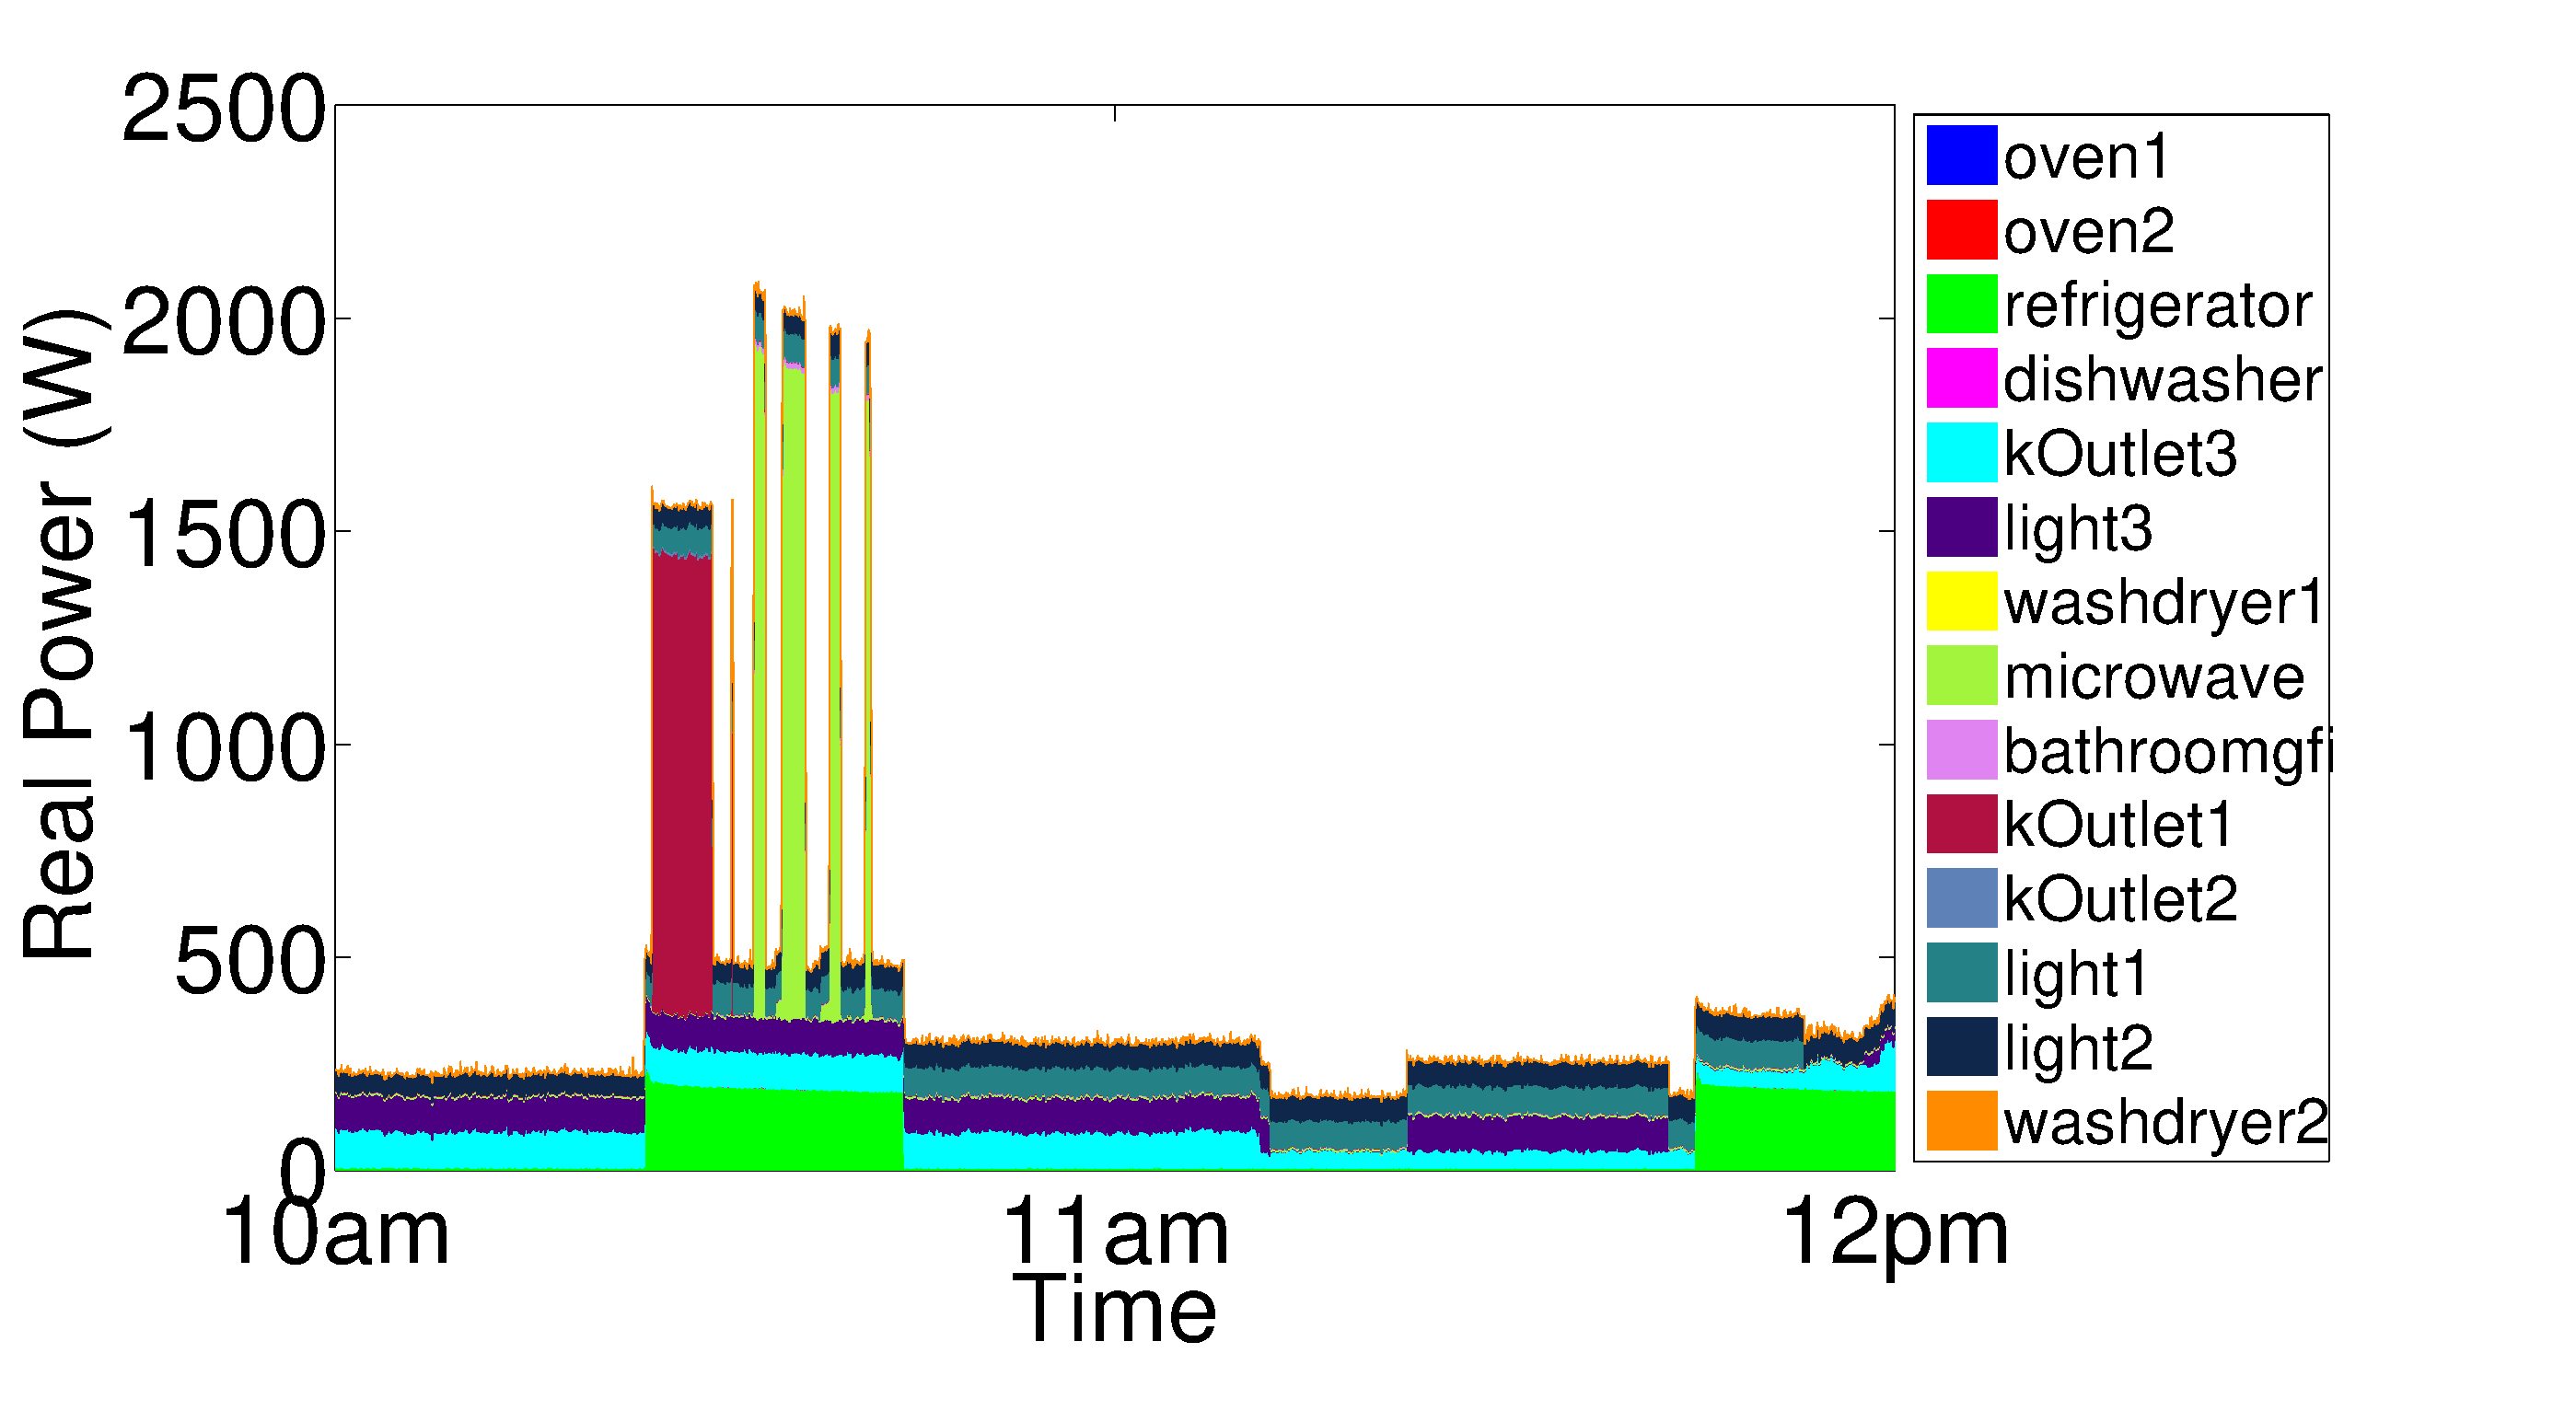
\includegraphics[width=0.5\textwidth]{figs/truth_disagg.pdf}\tabularnewline
   (a) & (b) \tabularnewline
    \end{tabular}
    }
	\caption{ (a) Aggregate power input to a disaggregation
algorithm. (b) Disaggregated information
about devices and their power usage patterns.}
	\label{fig_energyDisaggDefinition}
\end{figure*}

Energy disaggregation research can be understood in terms of 
the {\em features} that can be extracted from power measurements and
the underlying {\em algorithms} used.

One way to think of {\it features}
is in terms of
the sampling frequency
of meters. Low sampling frequency data is typically sampled at less than
$1$ Hz, while high sampling frequency data is sampled at higher than $1$ Hz.
Some features derivable from low frequency data are real power, reactive power,
low-order harmonics, and time of day. In addition to the ones inferable from
low frequency data, features from high frequency data include
many more characteristics such as harmonics, and current or voltage waveforms.

Another way to distinguish features is as transient vs steady state features.
Transient state features are only available from high frequency data. 
These features relate to transitory behavior seen in the current and voltage
waveforms when a device is turned on or off. 
On the other hand, steady state features are stable features that persist
after a device has changed its state. These
can be obtained from both low sampling frequency data and high sampling
frequency data. 

Yet another way to classify features is in terms of
AC power and non-AC power.
AC power characteristics are related to
current or voltage,
whereas non-AC power features include
power line noises, device correlation, and
contextual features like time or date, or weather information.

Initially, only
AC power features such as real power
and reactive power were studied~\cite{hart1992}.
With advances in electrical meter technology and availability of less expensive meters,
the transient state generated when a device turns on or off could be recorded and used
to identify devices~\cite{shaw2000PhdThesis}. 
Further, the raw current waveform~\cite{srinivasan2006neural}, voltage waveform~\cite{lam2007novel}, 
and the transform of the current waveform~\cite{chan2000harmonics}
can also be exploited as features.
Harmonics of non-linear devices
have also been studied~\cite{chan2000harmonics}.
Non-AC power features, such as power line noises~\cite{patel2007flick},
time of day, and device correlations~\cite{kim2011unsupervised}
are often combined with AC power features in modern systems. 

{\it Algorithms} applicable to energy disaggregation
can be categorized into supervised learning algorithms, 
unsupervised learning algorithms, and semi-supervised learning algorithms. 
%The applied data mining algorithms are composed of
%supervised learning algorithms, unsupervised learning algorithms
%and semi-supervised learning algorithms.
The supervised learning algorithms include
kNN methods~\cite{shaw2000PhdThesis},
support vector machines~\cite{patel2007flick},
neural networks~\cite{roos1994using},
genetic programming~\cite{baranski2004genetic},
sparse coding~\cite{kolter2010sparse}, 
as well as
combinations of supervised learning algorithms~\cite{nakano2007non}. 
Optimization algorithms used in the area of energy disaggregation have
been drawn from integer programming~\cite{suzuki2008nonintrusive}, 
dynamic programming~\cite{baranski2004detecting}, and
the Viterbi algorithm~\cite {zeifman2011viterbi}.
Unsupervised learning algorithms
have only been recently used in
 the last few years, and include
hierarchical clustering~\cite{gonccalves2011unsupervised},
factorial hidden Markov models (FHMMs)~\cite{kim2011unsupervised},
additive factorial approximate MAP (AFAMAP)~\cite{kolter2012aistat}, 
difference FHMM~\cite{parson2012nonintrusive}, 
and motif mining~\cite{shao2013temporal}.
Semi-supervised learning 
algorithms~\cite{lam2007novel,johnson2012bayesian} have also
been proposed.
%Because of the speciality of electricity,
%signal processing algorithm wavelet transform \cite{chan2000harmonics} is
%also an effectively adopted method.


\subsection {Challenges}
The field of energy disaggregation has evolved
over the last twenty years; while
some applications have achieved
qualified success, there are several challenging
problems that still need to be addressed before energy disaggregation can be
used more widely. Some of these problems include:

\begin{enumerate}
\item The number of devices is typically unknown and can only be
approximately estimated based on background information.

\item The number of power levels of each device is unknown.
Some devices such as lights may have only two steady states, viz. on and off.
Other devices  have several steady states.
For example, a microwave can operate in the states of defrost,
heat with low power, or heat with high power. Estimating
the exact number of states of a device is a hard problem.

\item Several devices may share the same real power and
it is hard to distinguish these devices from only the recorded aggregated
power values. 
For example, a light and a monitor could consume the same amount of real
power (e.g., around 38W). With more devices that share the same real power,
additional features are necessary to disambiguate among them.

\item Many devices may turn on or off at the same time.
A PC and printer likely turn on and off together, 
thus making it difficult to separate them from the aggregated power profile.

\item Instead of having a discrete range of power
levels, there are devices whose power consumption levels
   vary continuously, e.g.,
  variable speed devices (VSD), and lights with dimmers.
Once their power usage is aggregated with that from other devices, the
disaggregation problem becomes increasingly difficult.

\item Some devices are always on and seldom operated by
users. Because the operations on these devices are
rare, it is hard to identify these devices from prior historical data.

\end{enumerate}

The above problems are exacerbated in the case of commercial buildings.
While the voltage in residential buildings is typically $110$ or $220$ volts, 
the voltage in commercial buildings is
traditionally higher, at $208$ or $460$ volts.
Three-phase power is usually split
into single phase or two phases before reaching residential buildings.
In contrast, commercial buildings commonly use three phases.
Further, the devices in these two types of buildings are different.
Residential buildings
usually have devices such as microwaves,
refrigerators, ovens, lights, washers/dryers, and
air-conditioners.
The start-up duration of these devices
is short before they come to steady states.
Commercial buildings install more VSDs
including heating, ventilation, and air conditioning (HVAC) systems, 
variable-speed motor devices, and dimmable lighting. 
Further, banks of lights typically connect into a circuit together and
are powered on/off at the same time.

Generally, we face greater challenges in commercial buildings
than in residential buildings.
Norford and Leeb study non-intrusive load monitoring
challenges for commercial buildings~\cite{norford1996non}.
First,  load detection in commercial buildings is harder
because there are many devices powered on and off together.
Second, the start-up transient state of devices in commercial building is
much longer than those in discrete devices,
which dominate residential buildings.
Finally, in commercial buildings, reactive power is reduced to
make loads resistive, such as fluorescent lamp fixtures.

%The more devices connect,
%the possibility of case 2, case 3 and case 4 increases,
%the harder it is to disaggregate all devices correctly.

\subsection{Scope of this Survey}
Our objective is to provide an introduction to this space for a data
mining audience. While surveys exist on energy disaggregation,
e.g.,~\cite{zeifman2011nonintrusive},~\cite{liang2010load}, and~\cite{zoha2012survey}, they are mostly aimed at an electrical engineering audience and are
not suitable for data mining practitioners. Our survey provides both 
the background knowledge necessary and an overview of all aspects of
machine learning and data mining as applied to energy disaggregation.

In all survey papers, it is helpful to scope out what the survey does {\it not}
cover. The problem of disaggregation resurfaces in the
context of other utilities besides electricity, e.g.,
water~\cite{dai2011multi}, 
natural gas~\cite{froehlich2011disaggregated}, and music~\cite{schmidt2006nonnegative}. We do not cover these domains here and focus exclusively on electricity.
Second, there are many problems that appear related at first glance,
e.g., blind source separation~\cite{blumensath2005shift,davies2007source,lewicki2000learning} but are quite distinct from disaggregation. In the case of blind
source separation, the goal is to separate sources from at least as many
observations whereas in the case of disaggregation, only one aggregate signal
is provided. We do not cover these areas here.

\subsection{Organization}
The contents of this survey are organized as follows.
In Section~\ref{sec:basic}, we introduce some basic conceptions
of power, electricity, and electrical devices.
Next, in section~\ref{sec:problem},
we list several historical definitions of energy disaggregation
and present our working definition for the survey.
Characteristics which are used
to disaggregate devices are categorized in Section~\ref{sec:features}. 
It also describes how to setup an experimental testbed
and record necessary data with meters.
Section~\ref{sec:algorithms} summarizes a range of
algorithms that have been historically used for
energy disaggregation.
Section~\ref{sec:evaluation} takes up the important aspect of
defining evaluation measures for disaggregation.
Section~\ref{sec:ongoing} enumerates some tools, datasets, and software available to data mining researchers. Finally,
Section~\ref{sec:conclusion} identifies
promising research direction in this space.



